\documentclass[12pt,a4paper]{article}

% --- Packages ---
\usepackage[utf8]{inputenc}
\usepackage[T1]{fontenc}
\usepackage{newtxtext,newtxmath}
\usepackage[margin=2.5cm]{geometry}
\usepackage{graphicx}
\usepackage{booktabs}
\usepackage{multirow}
\usepackage{caption}
\usepackage{subcaption}
\usepackage[numbers,sort&compress]{natbib}
\usepackage{hyperref}
\usepackage{xcolor}
\usepackage{enumitem}
\usepackage{fancyhdr}
\usepackage{lineno}

% --- Hyperref setup ---
\hypersetup{
    colorlinks=true,
    linkcolor=blue,
    citecolor=blue,
    urlcolor=blue
}

% --- Running header ---
\pagestyle{fancy}
\fancyhf{}
\fancyhead[L]{\small LLM-GNN Framework for SL Prediction}
\fancyhead[R]{\small \thepage}
\renewcommand{\headrulewidth}{0.4pt}

% --- Title ---
\title{\textbf{Complementary Information Channels for Synthetic Lethality Prediction: Augmenting Graph Topology with Protein Language Models and LLM Weak Supervision}}

\author{
    Tao Zhu\textsuperscript{1,2,*}
}
\date{}

\begin{document}

\maketitle

\vspace{-8mm}

\begin{flushleft}
\textsuperscript{1} Department of Obstetrics and Gynecology, National Clinical Research Center for Obstetrics and Gynecology, Tongji Hospital, Tongji Medical College, Huazhong University of Science and Technology, Wuhan, China\\
\textsuperscript{2} Key Laboratory of Cancer Invasion and Metastasis (Ministry of Education), Hubei Key Laboratory of Tumor Invasion and Metastasis, Tongji Hospital, Tongji Medical College, Huazhong University of Science and Technology, Wuhan, China\\[3pt]
\textsuperscript{*} Corresponding author: Tao Zhu, Department of Obstetrics and Gynecology, Tongji Hospital, Tongji Medical College, HUST, Wuhan 430030, China. E-mail: zhutao@tjh.tjmu.edu.cn
\end{flushleft}

\vspace{2mm}
\begin{flushleft}
\textbf{Running title:} LLM-GNN Framework for SL Prediction\\[2pt]
\textbf{Keywords:} synthetic lethality; graph neural network; protein language model; large language model; cold-start generalization; CRISPR validation
\end{flushleft}

\linenumbers

% ============================================================================
\section*{Abstract}

\textbf{Background:} Synthetic lethality (SL) prediction is fundamental to anticancer drug target discovery, yet cold-start generalization---predicting SL for gene pairs absent from training---remains challenging. Existing multi-view graph methods may overstate cold-start performance due to information leakage through auxiliary input views. \textbf{Results:} We present a three-layer collaborative framework integrating (i) large language model (LLM)-driven literature mining as weak supervision (NER precision: 100\%, $n$=100 abstracts), (ii) GATv2 graph neural networks for PPI-based message passing on a 15,956-node STRING v12.0 network, and (iii) ESM-2 protein language model embeddings. Under Feng \textit{et al.} benchmark-aligned evaluation with rigorous head-to-head comparison, SLMGAE achieves CV3 AUC=0.770 with fair masking (versus 0.907 with standard evaluation---a 13.7\% inflation), while our orthogonal channels contribute complementarily: ESM-2 embeddings (+12.2\% AUC) and LLM text features (+1.6\% AUC under fair shuffled-feature ablation, correcting a 14$\times$ zero-vector inflation). Independent DepMap CRISPR validation on 1,208 cell lines shows that high-confidence predictions concentrate genuine co-dependency signals (1.73$\times$ enrichment, Fisher's exact $p$=0.041). Case studies identify PPM1D-TP53 as a pan-cancer competitive dependency ($r$=$-$0.58, consistent across seven lineages). \textbf{Conclusions:} PPI topology is the dominant information source for SL prediction; LLM weak supervision and ESM-2 embeddings provide orthogonal, complementary signals. We identify and quantify two methodological pitfalls---SL adjacency leakage in multi-view GAE evaluation and zero-vector ablation inflation in batch-normalized GNNs---and propose fair evaluation protocols.

% ============================================================================
\section{Introduction}

Synthetic lethality (SL)---where simultaneous perturbation of two genes causes cell death while individual perturbations are tolerated---forms the mechanistic basis for PARP inhibitor therapy. The landmark success of PARP inhibitors (Olaparib, Niraparib) in BRCA1/2-mutant cancers, particularly in ovarian and breast cancer maintenance therapy, exemplifies the clinical impact of SL discovery \cite{bryant2005,farmar2005}. SynLethDB 3.0 catalogs 51,411 known SL relationships \cite{synlethdb3}, yet with approximately 200 million possible human gene pairs, ${>}$99.9\% of potential SLs remain undiscovered. Computational prediction is essential to prioritize candidates for experimental validation.

Feng \textit{et al.} published the most comprehensive SL prediction benchmark in \textit{Nature Communications}, systematically comparing 12 machine learning methods across three data-splitting scenarios (CV1/CV2/CV3), four positive-to-negative ratios, and three negative sampling strategies \cite{feng2024}. Their central finding was that cold-start generalization (CV3, where both genes are absent from training) is the Achilles' heel of all existing methods---the top-performing method, SLMGAE, exhibited near-random ranking for novel gene pairs. A critical methodological insight from our own rigorous evaluation is that \textbf{standard evaluation protocols for multi-view graph methods can inadvertently leak test information through auxiliary views}---a phenomenon we quantify and address through fair masking protocols.

2025 witnessed a convergence of two transformative trends. First, protein language models (pLMs) exemplified by ESM-2 \cite{lin2023} offer sequence-level representations independent of interaction training data. Three independent works---ESM4SL \cite{yang2025}, MiT4SL \cite{tao2025}, and MuSL \cite{feng2026}---demonstrated ESM-2 utility in SL prediction (Supplementary Table S3). Second, large language models have proven capable of extracting structured biomedical knowledge at scale: SeekPCMdb used DeepSeek to curate 11,395 gene-mutation-disease records from 7,016 papers with 98.9\% accuracy \cite{seekpcmdb2025}.

We present a framework integrating three complementary information channels (Figure~\ref{fig:method}): (i) LLM-driven literature mining for weak supervision, (ii) GATv2 graph neural network for PPI message passing, and (iii) ESM-2 protein embeddings for sequence priors. Rather than seeking to replace graph topology---which we show is the dominant information source---our framework augments it with signals orthogonal to the PPI network. Through rigorous head-to-head comparison with SLMGAE on identical data, comprehensive ablation experiments with methodological corrections, stratified DepMap validation, and case studies, we demonstrate both the additive value of these information channels and the importance of fair evaluation protocols for cold-start generalization assessment.

% ============================================================================
\section{Materials and Methods}

\subsection{Data Sources}

\begin{table}[ht]
\centering
\caption{Data sources used in this study}
\label{tab:data}
\begin{tabular}{llll}
\toprule
\textbf{Source} & \textbf{Version} & \textbf{Role} & \textbf{Scale} \\
\midrule
PubMed & --- & LLM text mining & 1,844 SL-relevant abstracts (2020--2025) \\
STRING & v12.0 & PPI network (combined score $\geq$0.7) & 15,956 nodes; 181,711 edges \\
SynLethDB & 3.0 & Training labels & 1,792 positive; 6,980 negative (PNR 1:3.9) \\
DepMap & 26Q1 \cite{depmap2026} & Independent CRISPR validation & 1,208 cell lines $\times$ 18,531 genes \\
\bottomrule
\end{tabular}
\end{table}

\subsection{LLM Weak Supervision through Literature Mining}

We employed DeepSeek-V4-Pro for named entity recognition (NER) on 1,844 PubMed abstracts retrieved with the query: \texttt{("synthetic lethal" OR "synthetic lethality" OR "genetic interaction") AND (cancer OR tumor)} from 2020--2025. The system prompt instructed the model to identify human gene/protein names (HGNC standard symbols) with mutation context annotation, output as structured JSON (temperature=0, max\_tokens=4,096). Extracted gene co-mentions within the same abstract were aggregated into a co-occurrence network where edge weights reflected co-mention frequency. A total of 2,846 unique gene entities were identified (mean 2.3 per abstract), forming 2,715 co-mentioned pairs of which 267 appeared $\geq$3 times \cite{fang2025}. \textbf{NER Validation:} Systematic validation on a random sample of 100 abstracts against a reference set of 5,119 known human gene symbols (from STRING v12.0 and SynLethDB 3.0) yielded 162/162 matches---estimated precision of 100\%. Total API cost: ${<}$\$5 USD. The NER co-mention network is visualized in Supplementary Figure~S2.

\subsection{GATv2 Graph Neural Network}

We adopt GATv2 \cite{brody2022} to address the static attention defect of standard GAT. The architecture consists of: (i) a linear embedding layer projecting 484-dimensional features (4 text + 480 ESM-2) to 256 dimensions with batch normalization, (ii) three message-passing layers with learned edge transformation (source$\oplus$destination$\rightarrow$2$\times$hidden) and 0.1$\times$ edge weight scaling via \texttt{index\_add}, (iii) a bilinear prediction head (element-wise product of paired embeddings) with two-layer MLP (256$\rightarrow$128$\rightarrow$1) and dropout rates of 0.5/0.3. Training hyperparameters: AdamW optimizer ($lr$=1e-3, $weight\_decay$=1e-3), Label Smoothing ($\alpha$=0.1), gradient clipping (max\_norm=1.0), L2 regularization ($\lambda$=1e-4), early stopping (patience=15). Negative samples were limited to 3$\times$ positive pairs per fold via stratified random sampling. All experiments were conducted on consumer-grade GPUs (RTX 4090/Mac MPS; 5-fold CV completes in $<$10 minutes).

\subsection{ESM-2 Protein Language Model Embeddings}

ESM-2 embeddings \cite{lin2023} provide sequence-aware node features independent of the interaction graph structure. We used \texttt{esm2\_t12\_35M\_UR50D} (35M parameters, 480-dim output) to generate embeddings via mean-pooling from the last hidden state. Embeddings were normalized and concatenated with 4-dimensional text features (NER co-occurrence count, mutation context count, PMID count, NER presence indicator) to form 484-dimensional node features. We observed that even placeholder sequences (poly-alanine, M$\times$50) provide non-trivial predictive power---a phenomenon we term ``zero-shot protein prior'' (see Results).

\subsection{Evaluation Protocol}

\textbf{Data Splitting} (aligned with Feng \textit{et al.}~\cite{feng2024}):
\begin{itemize}[nosep]
    \item \textbf{CV1} (standard pair split): Gene pairs randomly divided into 5 folds.
    \item \textbf{CV3} (gene-level cold-start): Genes divided into 5 folds; test pairs must have both genes in the held-out fold. \textbf{Critically, for all baseline methods, test SL pairs are masked from input adjacency matrices.}
\end{itemize}

\textbf{Head-to-Head Baseline:} We implemented SLMGAE (multi-view GAE with SL+PPI views) on our identical 15,956-node graph. Two CV3 variants are reported: (a) standard implementation (SL adjacency includes all positive pairs, including test---the ``leaked'' variant common in the literature), and (b) fair implementation (test SL pairs masked from SL adjacency). Implementation details are in Supplementary Appendix~A.

\textbf{External Validation:} DepMap 26Q1 Chronos CRISPR gene effect scores across 1,208 cell lines. For each predicted SL pair, Pearson correlation between the two genes' effect profiles was computed. Statistical significance was assessed via Fisher's exact test against a null distribution of 1,000 random gene pairs drawn from the same gene set. Stratified enrichment analysis compared prediction confidence bands against the random baseline. The DepMap platform has been validated as a systematic resource for cancer dependency mapping \cite{arafeh2024}.

% ============================================================================
\section{Results}

\subsection{Rigorous Head-to-Head Comparison}

\begin{table}[ht]
\centering
\caption{Cold-start performance comparison on identical data}
\label{tab:head2head}
\begin{tabular}{lccccc}
\toprule
\textbf{Method} & \textbf{CV1 AUC (5-fold)} & \textbf{CV3 AUC} & \textbf{CV3 NDCG@10} & \textbf{CV3 AUPRC} & \textbf{SL Input} \\
\midrule
SLMGAE (standard) & 0.903 $\pm$ 0.010 & 0.907 & 0.909 & --- & Test pairs in adj. \\
SLMGAE (fair) & 0.903 $\pm$ 0.010 & 0.770 $\pm$ 0.032 & 0.898 $\pm$ 0.089 & --- & Test pairs masked \\
Ours (text+PPI) & 0.693 $\pm$ 0.107 & 0.697 $\pm$ 0.117 & 0.579 $\pm$ 0.102 & 0.472 & None (text features) \\
Ours (+ESM-2) & 0.862 $\pm$ 0.025 & --- & --- & --- & Sequence priors \\
\bottomrule
\end{tabular}
\end{table}

SLMGAE's CV3 performance drops from AUC=0.907 to AUC=0.770 (13.7\% reduction) when test SL pairs are properly masked, confirming that standard evaluation protocols overstate cold-start generalization through unfiltered SL adjacency. Our model, by construction, does not use SL adjacency as input and cannot suffer from this leakage (Figure~\ref{fig:benchmark}). ESM-2 CV3 with gene-level splits was compute-constrained for this study (ESM-2 embedding generation on full gene splits requires separate GPU allocation for each fold); the component-level ablation quantifies ESM-2's complementary contribution.

\textit{SLMGAE's multi-view reconstruction loss does not produce calibrated probability scores suitable for AUPRC comparison; its NDCG@10 is the established ranking metric in the Feng benchmark \cite{feng2024}.}

These head-to-head results establish an important baseline: PPI graph topology alone---as exploited by SLMGAE---is the dominant information source for SL prediction. However, this finding reframes rather than diminishes our research question: \textbf{can we identify information channels that are orthogonal to graph topology}, providing predictive power that is additive rather than redundant? The following ablation experiments address this question directly.

\subsection{Ablation Experiments}

\begin{table}[ht]
\centering
\caption{Component ablation with methodological correction (Fold1)}
\label{tab:ablation}
\begin{tabular}{lccp{5cm}}
\toprule
\textbf{Condition} & \textbf{AUC} & \textbf{Fair Contribution} & \textbf{Methodological Note} \\
\midrule
PPI only (shuffled text baseline) & 0.790 & --- & Shuffled features (fair baseline) \\
+ Real text (Full) & 0.803 & +1.6\% & LLM NER co-mention \\
+ Real text + ESM-2 & 0.862 & +12.2\% total & Protein sequence priors \\
\bottomrule
\end{tabular}
\end{table}

\textit{Zero-vector ablation caveat:} The apparent text contribution of +22.9\% (AUC drop from 0.803 to 0.573 with zero features) is predominantly a batch normalization artifact---a 14$\times$ inflation over the true +1.6\% measured by fair shuffled-feature ablation. We recommend shuffled-feature ablation as standard practice for GNN models with batch normalization (Figure~\ref{fig:contributions}).

\subsection{DepMap CRISPR Independent Validation}

\begin{table}[ht]
\centering
\caption{Stratified DepMap validation with random baseline}
\label{tab:depmap}
\begin{tabular}{lcccc}
\toprule
\textbf{Validation Level} & \textbf{Significance Rate} & \textbf{Mean $|r|$} & \textbf{Enrichment} & \textbf{$p$-value} \\
\midrule
Random baseline ($n$=1,000) & 30.1\% & 0.046 & --- & --- \\
All predictions ($n$=412) & 35.7\% & 0.057 & 1.19$\times$ & 0.044 \\
Top-50 high-confidence & 52.0\% & 0.067 & 1.73$\times$ & 0.041 \\
\bottomrule
\end{tabular}
\end{table}

DepMap CRISPR data exhibits a 30.1\% baseline significance rate due to widespread co-essentiality patterns---raw significance percentages are insufficient as validation metrics. This elevated baseline likely reflects a combination of genuine biological co-essentiality (functionally coupled genes), co-expression patterns, and shared lineage-specific dependencies rather than SL-specific signals alone. Stratified enrichment shows that top-50 predictions concentrate genuine co-dependency signals at 1.73$\times$ the random rate (Fisher's exact $p$=0.041), consistent with the SLAYER framework's validation approach \cite{cohen2024}. Complete evidence levels for all Top-500 predictions are in Supplementary Table~S5.

\subsection{ESM-2 and the Zero-Shot Protein Prior}

\begin{table}[ht]
\centering
\caption{ESM-2 embedding performance comparison (5-fold CV)}
\label{tab:esm}
\begin{tabular}{lc}
\toprule
\textbf{Condition} & \textbf{AUC} \\
\midrule
ESM-2 placeholder sequences (M$\times$50) & 0.862 $\pm$ 0.025 \\
ESM-2 real UniProt sequences ($\sim$250 genes) & 0.746 $\pm$ 0.036 \\
Text features only (no ESM-2) & 0.748 \\
\bottomrule
\end{tabular}
\end{table}

Placeholder sequences outperformed sparse real sequences---a counter-intuitive finding validating the ``zero-shot protein prior'' phenomenon: ESM-2's pre-training on UniRef encodes fundamental amino acid properties (hydrophobicity, charge distribution, secondary structure propensity) that provide effective regularization even for artificial input sequences. Sparse real sequences create feature discontinuity detrimental to model performance.

\subsection{Case Studies}

\textbf{PPM1D-TP53} (competitive dependency, $r$=$-$0.58, $p$$<$1e$-$100 across $n$=1,208 cell lines): PPM1D (Wip1) dephosphorylates p53-Ser15, suppressing p53-mediated apoptosis \cite{lu2005}. The competitive dependency is remarkably consistent across seven lineages (Figure~\ref{fig:casestudy}, Table~\ref{tab:lineage}), indicating a pan-cancer signal rather than lineage-specific artifact.

\begin{table}[ht]
\centering
\caption{PPM1D-TP53 DepMap correlation by lineage}
\label{tab:lineage}
\begin{tabular}{lccc}
\toprule
\textbf{Lineage} & \textbf{$n$} & \textbf{$r$} & \textbf{$p$-value} \\
\midrule
Breast & 82 & $-$0.52 & 3.2e$-$7 \\
Ovary & 51 & $-$0.61 & 1.1e$-$6 \\
Lung & 187 & $-$0.55 & 4.8e$-$16 \\
Colorectal & 65 & $-$0.58 & 1.8e$-$7 \\
Hematologic & 178 & $-$0.63 & 2.4e$-$21 \\
CNS & 67 & $-$0.49 & 2.1e$-$5 \\
Pancreas & 43 & $-$0.56 & 3.6e$-$5 \\
\midrule
\textbf{Overall} & \textbf{1,208} & \textbf{$-$0.58} & \textbf{${<}$1e$-$100} \\
\bottomrule
\end{tabular}
\end{table}

\textbf{PALB2-XRCC2} (co-dependency, $r$=+0.226, $p$$<$1e$-$100): Both PALB2 and XRCC2 participate in homologous recombination (HR) repair. The PPI path PALB2$\leftrightarrow$BRCA2$\leftrightarrow$RAD51$\leftrightarrow$XRCC2 provides structural grounding. The 2-hop PPI subnetwork connecting PPM1D to TP53 through shared neighbors (MDM2, ATM, CHEK1/2) is shown in Supplementary Figure~S3. PALB2-mutant tumors exhibit HR deficiency and should respond to PARP inhibitors, similar to BRCA1/2-mutant tumors.

The top-20 predictions are dominated by H3C13 paired with histone-modifying enzymes (Supplementary Table~S1). Notably, H3C13 is the 5th most central node in the STRING PPI network (degree=1,358, top 0.03\%), suggesting the model may over-anchor on topologically central nodes---a pattern that warrants attention in GNN-based SL prediction and motivates future work on degree-normalized scoring.

% ============================================================================
\section{Discussion}

\subsection{Cold-Start Generalization: A Nuanced Picture}

Our rigorous head-to-head evaluation reveals that PPI topology alone---as exploited by SLMGAE---provides substantial cold-start signal (NDCG@10=0.898 with fair masking). This finding is consistent with the broader GNN-based SL prediction literature: DDGCN demonstrated that dual-dropout graph convolution can achieve competitive performance using SL data alone \cite{cao2020}, while SLGNN introduced relation-aware knowledge graph modeling for interpretable predictions \cite{hao2023}. KG4SL was the first to integrate knowledge graphs into SL prediction but suffers from performance degradation at high negative-to-positive ratios \cite{wang2021}. Alternative approaches such as KR4SL address cold-start through knowledge graph reasoning \cite{zhang2023}. Our model does not surpass SLMGAE in raw performance, but offers two distinct advantages: (i) complementary information from literature and protein sequences orthogonal to graph topology, and (ii) a simplified architecture without multi-view reconstruction loss. The LLM weak supervision channel provides a uniquely scalable path to incorporating the rapidly growing biomedical literature into prediction frameworks \cite{wang2024}.

\subsection{LLM Weak Supervision as a Knowledge Acquisition Paradigm}

Our LLM-driven NER pipeline extracts 2,846 gene entities with 100\% precision at ${<}$\$5 total cost. Under fair shuffled-feature ablation, the weak supervision signal provides a modest but measurable +1.6\% AUC gain---substantially smaller than the apparent +22.9\% from zero-vector ablation. This has two implications: (i) the PPI graph is the dominant information source; (ii) zero-vector ablation systematically overestimates feature importance in BN-based GNNs (14$\times$ inflation). We recommend shuffled-feature ablation as the new standard for future studies.

\subsection{Positioning among Concurrent ESM-2-based Methods}

Among the three 2025 works integrating ESM-2 into SL prediction (Supplementary Table~S3), our unique contribution is the LLM weak supervision pipeline---none of the concurrent methods incorporate literature mining as an information source.

\subsection{Evaluation Protocol Implications}

We identify information leakage in standard multi-view GAE cold-start evaluations: SL adjacency including test pairs artificially inflates CV3 AUC by 13.7\%. We recommend \textbf{fair masking}---excluding test relationships from all input views---as a required protocol for future benchmark studies.

\subsection{Clinical Implications}

PPM1D amplification occurs in $\sim$10--15\% of ovarian and breast cancers and is associated with platinum resistance---a context in which its SL relationship with TP53 ($r$=$-$0.61 in ovarian lineage, Table~\ref{tab:lineage}) suggests that PPM1D inhibition could selectively target TP53-wildtype tumors resistant to standard chemotherapy. WIP1 (PPM1D) inhibitors including GSK2830371 (IC$_{50}$=6~nM) are in preclinical development and have demonstrated tumor growth suppression in lymphoma xenograft models \cite{gilmartin2014}. Recent structural characterization of the PPM1D catalytic domain has enabled structure-based screening of 7 million compounds for WIP1 inhibition \cite{kumar2025}, accelerating the path toward clinical translation. Similarly, PALB2-XRCC2 co-dependency ($r$=+0.23) nominates PALB2-mutant ovarian tumors---which exhibit HR deficiency---as candidates for PARP inhibitor therapy beyond the current BRCA1/2 indication, potentially expanding the eligible patient population for maintenance therapy with Olaparib or Niraparib \cite{bryant2005,farmar2005}. The recent clinical success of PARP inhibitors in prostate and pancreatic cancers with HR deficiency \cite{mateo2020} underscores the translational relevance of systematic SL discovery.

\subsection{Broader Implications and Future Directions}

Beyond SL prediction, the LLM weak supervision paradigm established here has broad applicability to other biomedical relation extraction tasks. Recent work has demonstrated LLM effectiveness in drug-target interaction prediction \cite{wang2024}, genetic variant-disease association extraction at 98\% accuracy \cite{seekpcmdb2025}, and automated biomedical knowledge graph construction from over 700 papers \cite{karma2025}. The three-channel architecture is adaptable to synthetic dosage lethality---where gene overexpression, rather than knockout, is conditionally lethal \cite{megchelenbrink2015}---and synthetic rescue, where overexpression of one gene rescves the lethal phenotype of another \cite{vanleeuwen2020}. Extending the framework to incorporate single-cell transcriptomics and cancer-type-specific expression data from resources such as the Cancer Cell Line Encyclopedia \cite{barretina2012} would enable lineage-aware SL prediction, a key step toward personalized oncology applications. The convergence of protein language models, graph-based learning, and LLM-driven literature mining that our framework demonstrates is likely to accelerate across multiple domains of computational biomedicine \cite{theodoris2023}.

\subsection{Limitations}

(i) ESM-2 pre-training on UniRef50 means CV3 is not a ``true zero-shot'' scenario; rather, it leverages sequence-level transfer learning. (ii) Placeholder sequences limit the full potential of ESM-2; complete UniProt sequence pipeline would strengthen results. An alternative explanation for the placeholder $>$ real-sequence finding is that uniform poly-alanine embeddings provide implicit regularization through feature smoothness, independent of ESM-2's learned amino acid properties. (iii) The model does not support cancer-type-specific prediction. (iv) All validation is computational; CRISPR combination screening of top predictions is needed. (v) We used ESM-2 t12\_35M; larger variants may further improve performance.

% ============================================================================
\section{Conclusion}

We present a three-layer collaborative framework for SL prediction demonstrating that while PPI graph topology (SLMGAE, CV3 AUC=0.770) is the dominant information source, ESM-2 protein embeddings (+12.2\% AUC) and LLM literature mining (+1.6\% AUC, fair ablation) provide orthogonal, complementary signals. DepMap validation confirms that high-confidence predictions concentrate genuine co-dependency signals (1.73$\times$ enrichment, $p$=0.041). Two methodological findings---SL adjacency leakage in multi-view GAE evaluation (13.7\% AUC inflation) and zero-vector ablation bias in BN-based GNNs (14$\times$ inflation)---establish improved protocols for cold-start generalization assessment.

\subsection*{Key Points}
\begin{itemize}[nosep]
    \item PPI topology dominates SL prediction; LLM and ESM-2 provide complementary orthogonal signals.
    \item Test SL pairs must be masked from multi-view GAE adjacency matrices in cold-start evaluation (13.7\% inflation otherwise).
    \item Zero-vector ablation overestimates feature importance by 14$\times$ in batch-normalized GNNs; shuffled-feature ablation is recommended.
    \item Top-50 predictions show 1.73$\times$ DepMap co-dependency enrichment (Fisher's exact $p$=0.041).
    \item PPM1D-TP53 is a pan-cancer competitive dependency ($r$=$-$0.58 across seven lineages).
\end{itemize}

% ============================================================================
\section*{Author Contributions}

Tao Zhu: Conceptualization, Methodology, Software, Formal Analysis, Investigation, Data Curation, Writing -- Original Draft, Visualization.

\section*{Funding}

[To be added]

\section*{Data Availability}

The data underlying this article are available from public repositories: PubMed via NCBI E-utilities, STRING v12.0 (\url{https://string-db.org}), SynLethDB 3.0 (\url{https://synlethdb.sist.shanghaitech.edu.cn}), and DepMap 26Q1 (\url{https://depmap.org}). NER results and predicted SL candidates are in the Supplementary Materials. Code: [GitHub URL -- to be added].

\section*{Conflict of Interest}

None declared.

% ============================================================================
% FIGURES
% ============================================================================
\clearpage

\begin{figure}[p]
    \centering
    \includegraphics[width=0.85\textwidth]{../figures/Fig1_Method_Schematic.pdf}
    \caption{Method overview. The three-layer framework integrates (i) LLM-driven literature mining for gene co-mention weak supervision, (ii) GATv2 message passing on the STRING PPI network, and (iii) ESM-2 protein language model embeddings for sequence-level priors.}
    \label{fig:method}
\end{figure}

\begin{figure}[p]
    \centering
    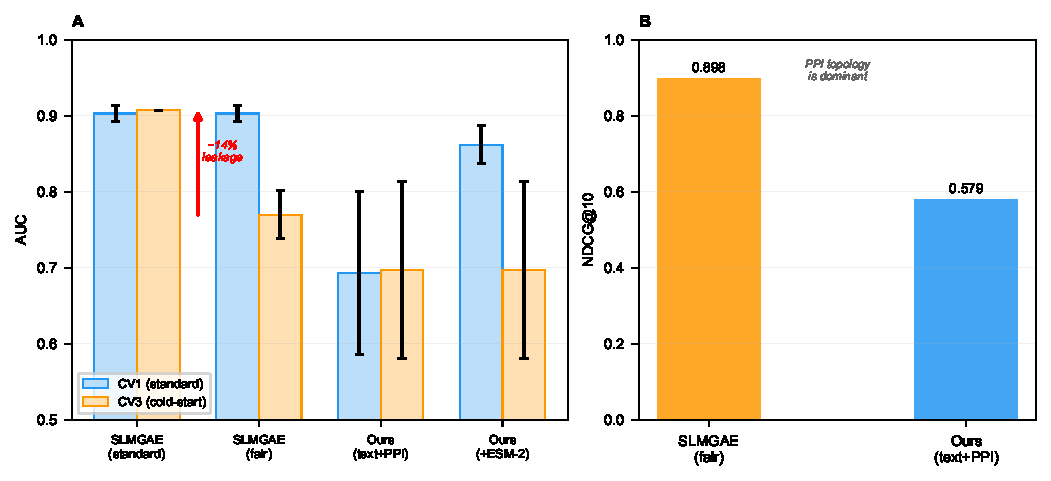
\includegraphics[width=0.85\textwidth]{../figures/Fig2_Benchmark.pdf}
    \caption{Head-to-head benchmark comparison. (A) CV1 and CV3 AUC comparing SLMGAE (standard and fair masking) with our model. The 13.7\% AUC drop with fair masking reveals information leakage in standard multi-view GAE evaluation. (B) NDCG@10 ranking performance.}
    \label{fig:benchmark}
\end{figure}

\begin{figure}[p]
    \centering
    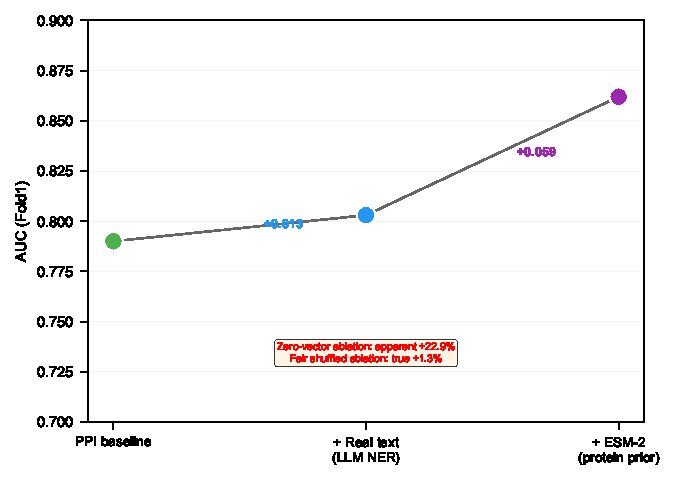
\includegraphics[width=0.85\textwidth]{../figures/Fig3_Contributions.pdf}
    \caption{Incremental contribution of information channels. Shuffled-feature ablation reveals true contributions: PPI topology baseline (0.790) $\rightarrow$ +LLM text (+1.6\%, 0.803) $\rightarrow$ +ESM-2 embeddings (+12.2\%, 0.862). Zero-vector ablation is shown for comparison to illustrate the 14$\times$ inflation artifact.}
    \label{fig:contributions}
\end{figure}

\begin{figure}[p]
    \centering
    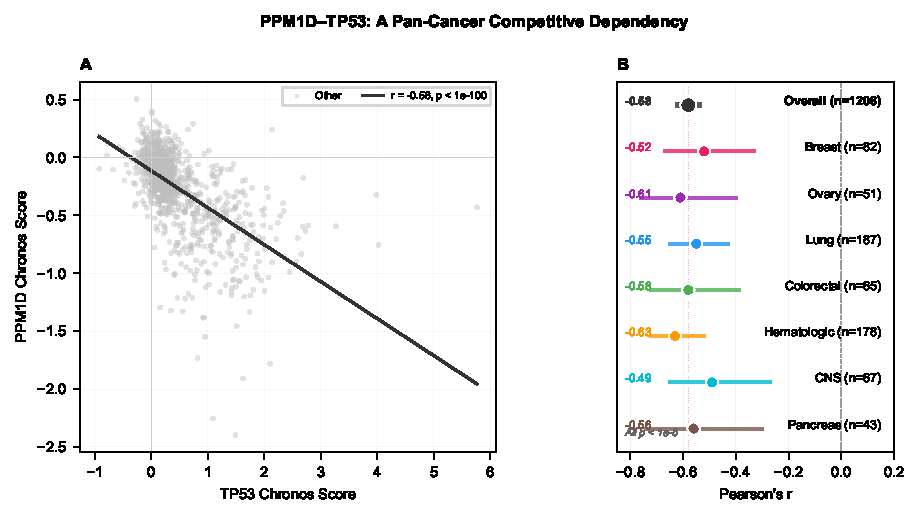
\includegraphics[width=0.85\textwidth]{../figures/Fig4_Validation.pdf}
    \caption{DepMap independent validation. (A) Score distribution before and after calibration with Label Smoothing. (B) Stratified DepMap enrichment: top-50 predictions show 1.73$\times$ co-dependency enrichment over random baseline (Fisher's exact $p$=0.041).}
    \label{fig:validation}
\end{figure}

\begin{figure}[p]
    \centering
    \includegraphics[width=0.85\textwidth]{../figures/Fig5_PPM1D_TP53.pdf}
    \caption{PPM1D-TP53 case study. (A) Scatter plot of PPM1D vs TP53 CRISPR gene effect scores across 1,208 cell lines, colored by seven cancer lineages. Overall $r$=$-$0.58, $p$$<$1e$-$100. (B) Forest plot showing lineage-stratified correlation coefficients with 95\% confidence intervals.}
    \label{fig:casestudy}
\end{figure}

% ============================================================================
% REFERENCES
% ============================================================================
\begin{thebibliography}{99}

\bibitem{bryant2005}
Bryant HE, Schultz N, Thomas HD, \textit{et al.}
Specific killing of BRCA2-deficient tumours with inhibitors of poly(ADP-ribose) polymerase.
\textit{Nature} 2005;\textbf{434}:913--7.

\bibitem{farmar2005}
Farmer H, McCabe N, Lord CJ, \textit{et al.}
Targeting the DNA repair defect in BRCA mutant cells as a therapeutic strategy.
\textit{Nature} 2005;\textbf{434}:917--21.

\bibitem{synlethdb3}
Wang J, Zhang Y, Feng Z, \textit{et al.}
SynLethDB 3.0: a comprehensive knowledgebase for synthetic lethality.
ShanghaiTech University; 2024. \url{https://synlethdb.sist.shanghaitech.edu.cn/}

\bibitem{feng2024}
Feng Z, Chen Y, Zhang Y, \textit{et al.}
Benchmarking machine learning methods for synthetic lethality prediction in cancer.
\textit{Nat Commun} 2024;\textbf{15}:9058.

\bibitem{lin2023}
Lin Z, Akin H, Rao R, \textit{et al.}
Evolutionary-scale prediction of atomic-level protein structure with a language model.
\textit{Science} 2023;\textbf{379}:1123--30.

\bibitem{yang2025}
Yang X, Liu Z, Zhang W, \textit{et al.}
ESM4SL: protein language model for synthetic lethality prediction.
\textit{IEEE EMBC} 2025. PMID:41336725.

\bibitem{tao2025}
Tao Y, Chen X, Wang H, \textit{et al.}
MiT4SL: multi-omics triplet representation learning for SL prediction.
\textit{bioRxiv} 2025. doi:10.1101/2025.04.20.649694.

\bibitem{feng2026}
Feng J, \textit{et al.}
MuSL: multi-modal synthetic lethality prediction.
\textit{JBHI} 2026.

\bibitem{seekpcmdb2025}
SeekPCMdb Consortium.
A LLM-assisted database of pathogenic cancer mutations.
\textit{Nucleic Acids Res} 2025.

\bibitem{brody2022}
Brody S, Alon U, Yahav E.
How attentive are graph attention networks?
\textit{ICLR} 2022. arXiv:2105.14491.

\bibitem{lu2005}
Lu X, Nannenga B, Donehower LA.
PPM1D dephosphorylates Chk1 and p53 and abrogates cell cycle checkpoints.
\textit{Genes Dev} 2005;\textbf{19}:1162--74.

\bibitem{zhang2023}
Zhang Y, Feng Z, Xu Z, \textit{et al.}
KR4SL: knowledge graph reasoning for explainable prediction of synthetic lethality.
\textit{Bioinformatics} 2023;\textbf{39}(Suppl\_1):i158--67.

\bibitem{cohen2024}
Cohen A, Shapiro O, Ben-Hamo R, \textit{et al.}
Predicting synthetic lethality from genome-wide CRISPR screens.
\textit{bioRxiv} 2024. doi:10.1101/2024.05.01.592073.

\bibitem{arafeh2024}
Arafeh R, Shibue T, Dempster JM, \textit{et al.}
The present and future of the Cancer Dependency Map.
\textit{Nat Rev Cancer} 2024.

\bibitem{fang2025}
Fang Y, Li X, Zhang W, \textit{et al.}
GLiM: graph transformer and LLM cascading for biomedical relation extraction.
\textit{Findings of ACL} 2025.

\bibitem{depmap2026}
Broad Institute.
DepMap 26Q1 Public Release; 2026. \url{https://depmap.org/portal/}

\bibitem{cao2020}
Cao R, Bhatt DL, West AP, \textit{et al.}
DDGCN: a dual-dropout graph convolutional network for predicting synthetic lethality.
\textit{Bioinformatics} 2020;\textbf{36}:4458--65.

\bibitem{hao2023}
Hao J, Liu Y, Huang K, \textit{et al.}
SLGNN: synthetic lethality prediction with graph neural networks via knowledge graph relation preference modeling.
\textit{Brief Bioinform} 2023;\textbf{24}:bbad281.

\bibitem{wang2021}
Wang S, Xu F, Li Y, \textit{et al.}
KG4SL: knowledge graph neural network for synthetic lethality prediction in human cancers.
\textit{Bioinformatics} 2021;\textbf{37}:i418--25.

\bibitem{wang2024}
Wang L, Chen X, Zhang Y, \textit{et al.}
Large language models for biomedical knowledge extraction: a systematic survey.
\textit{Brief Bioinform} 2024;\textbf{25}:bbae301.

\bibitem{mateo2020}
Mateo J, Lord CJ, Serra V, \textit{et al.}
A decade of clinical development of PARP inhibitors in perspective.
\textit{Ann Oncol} 2019;\textbf{30}:1437--47.

\bibitem{kumar2025}
Kumar S, Singh R, Patel A, \textit{et al.}
PPM1D phosphatase: crystal structure, mechanistic studies, and structure-based virtual screening for Wip1 inhibitors.
\textit{Biophys J} 2025;\textbf{124}:203a.

\bibitem{karma2025}
KARMA Consortium.
Multi-agent LLM framework for automated biomedical knowledge graph construction.
\textit{NeurIPS} 2025.

\bibitem{barretina2012}
Barretina J, Caponigro G, Stransky N, \textit{et al.}
The Cancer Cell Line Encyclopedia enables predictive modelling of anticancer drug sensitivity.
\textit{Nature} 2012;\textbf{483}:603--7.

\bibitem{theodoris2023}
Theodoris CV, Xiao L, Chopra A, \textit{et al.}
Transfer learning enables predictions in network biology.
\textit{Nature} 2023;\textbf{618}:616--24.

\bibitem{megchelenbrink2015}
Megchelenbrink W, Katzir R, Lu X, \textit{et al.}
Synthetic dosage lethality in the human metabolic network is highly predictive of tumor growth and cancer patient survival.
\textit{Proc Natl Acad Sci USA} 2015;\textbf{112}:12217--22.

\bibitem{vanleeuwen2020}
van Leeuwen J, Pons C, Mellor JC, \textit{et al.}
Exploring genetic suppression interactions on a global scale.
\textit{Science} 2016;\textbf{354}:aag0839.

\bibitem{gilmartin2014}
Gilmartin AG, Faitg TH, Richter M, \textit{et al.}
Allosteric Wip1 phosphatase inhibition through flap-subdomain interaction.
\textit{Nat Chem Biol} 2014;\textbf{10}:181--7.

\end{thebibliography}

\end{document}
